\documentclass{article}
\usepackage[utf8]{inputenc}
\usepackage[final]{pdfpages}

\title{Development Plan - Group 12}
\author{
  Safwan Hossain\\
  \texttt{hossam18}\\
  \and
  Tyler Magarelli\\
  \texttt{magarelt}\\
  \and
  Eamon Earl\\
  \texttt{earle2}
}

\date{February 4th, 2022}

\begin{document}

\maketitle

\section{Team Meeting and Communication Plan}

Our meeting plan will be to attend both of our lab sections, on Mondays and Thursdays. Mondays can be where we re-centralize our code and assign roles for the coming week, and Thursday sessions will be for checking in on progress and re-configuring workloads if need be. For tighter time crunches, a session on the weekend can be scheduled at a time that works for all team members. If a member has to miss a meeting, the minutes and important details will be provided to them, as well as their role for the week. 

Additionally, a rough UML dependency hierarchy will be incrementally developed throughout our meetings so that we can focus our efforts on working bottom-up through the hierarchy, minimizing 'ghost references' to unmade but expected modules.  

In terms of communication, we believe that teams is more than adequate in facilitating our meetings. Additionally, teammates will exchange numbers to ensure that they can always be reached, should the need arise.  


\section{Team Member Roles}

Due to the small size of the team, we have decided not to elect a project manager, opting instead for a democratic project hierarchy. Ultimately, under these circumstances in a group of three, the best ideas and priorities should still float to the top, as options that are deemed best by a majority of the group can be voted in two-to-one, ensuring that the project does not stagnate and that no one member can prioritize their ideas over any other. Additionally, for meetings we will document our ideas and our roles for that time frame on a google doc, where we can all see what was discussed and what is required from us on an individual basis.

\section{Git Workflow Plan}

We will be implementing a centralized workflow plan, wherein each member can take time during the meeting to summarize what they completed, push their code, so that any conflicts can be resolved as a group. We would like to ensure that by the end of every session, all changes have been centralized so that team members are pulling from identical source code for the next session.

The project workload will also be split up into individual tasks that can be assigned to each group member. Each task will be defined such that it has minimum dependency on any other tasks. This method will minimize the amount of merge conflicts that we may have when we combine our code during meetings. 

\section{Proof of Concept Demonstration Plan}

The most significant risks are implementing the GUI (guaranteed risk), and implementing online play, an optional source of risk that we have been seriously considering. Depending on whether or not we wish to pursue this option, which will be decided and finalized in our upcoming meetings, we will possibly need to demonstrate this online play. Regardless, our proof of concept will be a demo of the GUI, in either online or offline play, which will involve some degree of playability or simulation of a poker game. At that time, we may simply use a text-based GUI using the console, but later on it can be made using Unity and JavaScript. 


\section{Technology}

We will be programming in Java, and may use JavaScript for the development of the GUI. The technology required for online play (server integration), is yet to be determined, but will be considered in meetings to come. As of right now, we will be focusing on the core game-play. 


\section{Coding Style}

We will be programming in Java, and as such our hand is forced towards OOP. We will be implementing our program using the MVC (Model view.View Controller) architecture, as it is an ideal structure for playable games. In terms of heuristics for the programming itself, we will be prioritizing generality in our base code as well as designing for change, such that adding and implementing further forms of poker or even non-gambling card games will be exceptionally easy. This seems like the best course of action and the most logical, as every card game's model is identical; one deck of cards, and some variable hand size. Rules can be scripted in the particular controller for each game type, and new games could be added and created overnight. We will also be prioritizing run time over memory, as the memory required will be inherently low when the model is capped at 52 cards.

\section{Project Schedule}

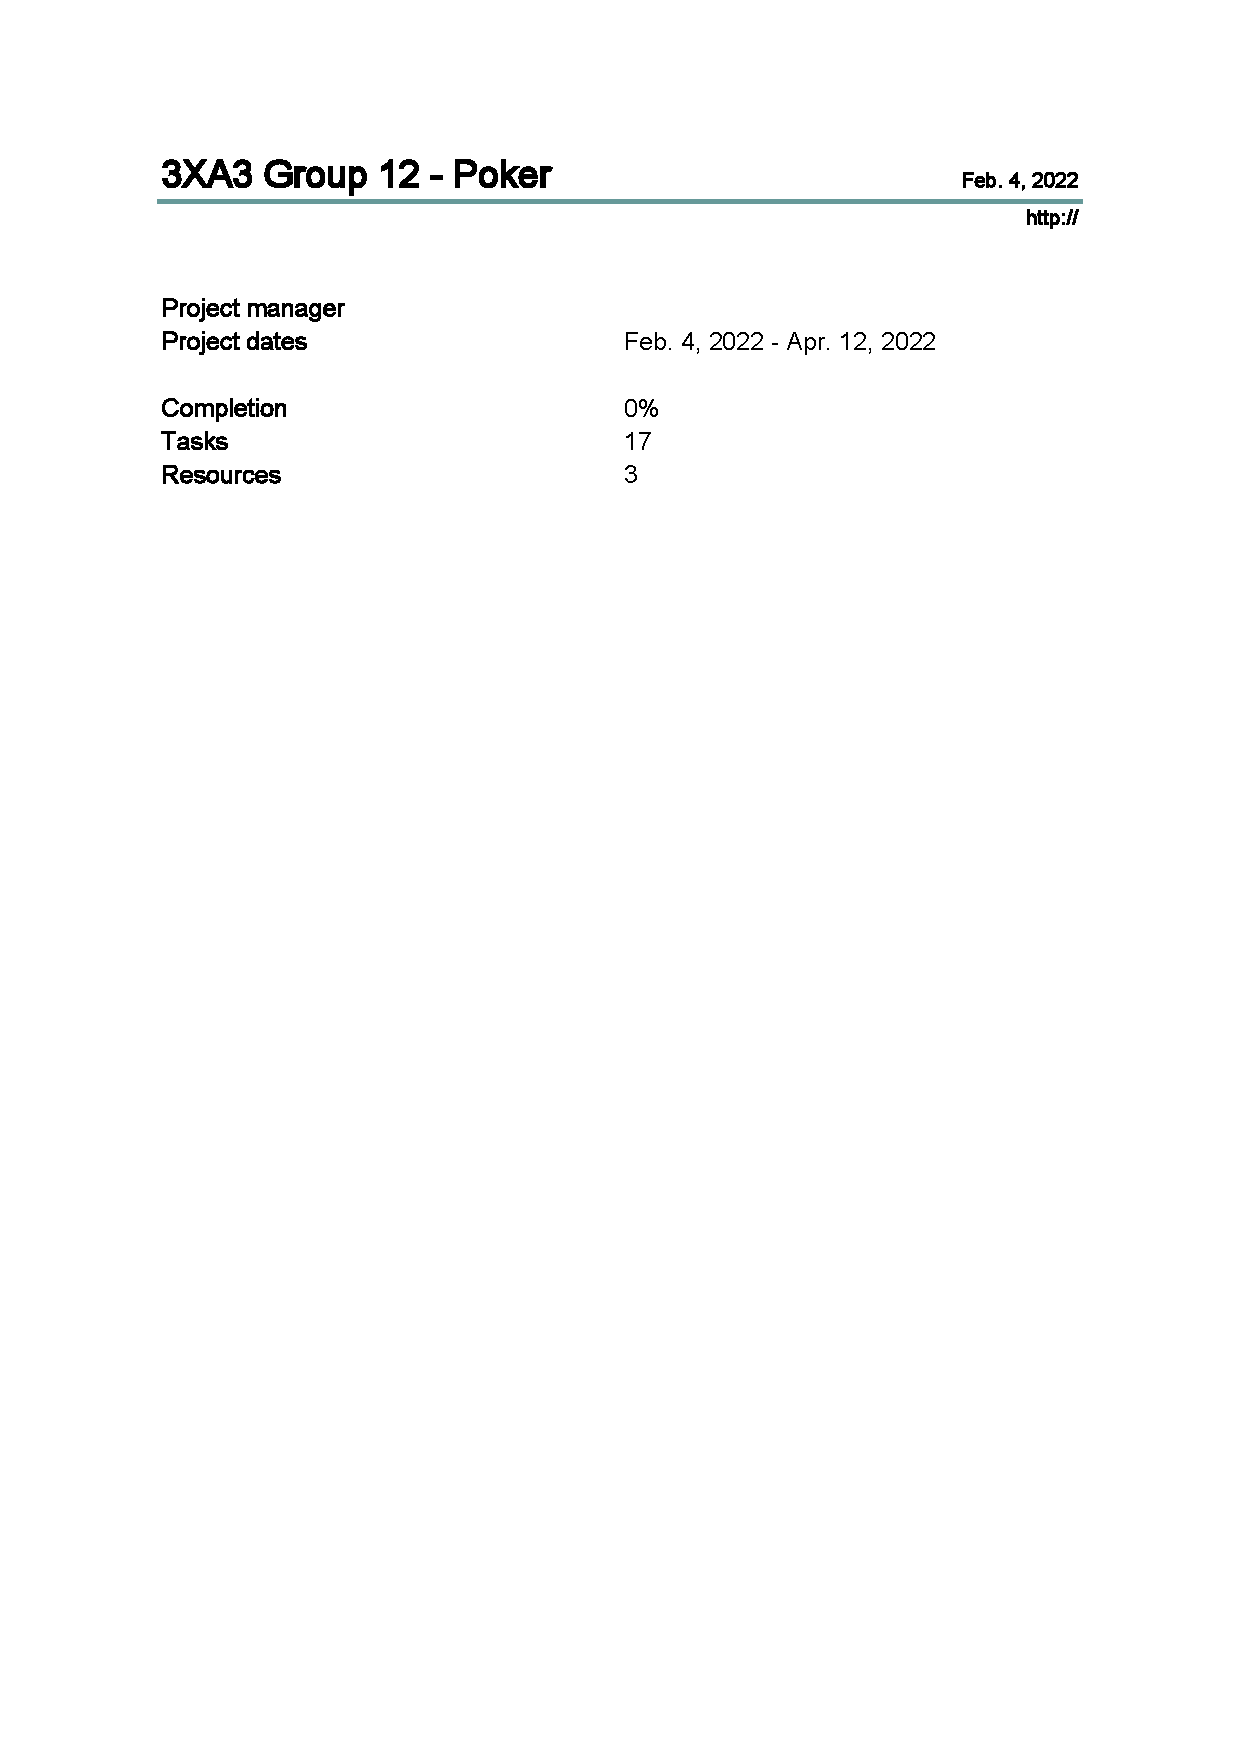
\includepdf[pages=-]{ProjectSchedule.pdf}

\section{Project Review}
**to be done at a later date**


\end{document}
